\documentclass[tikz,border=10pt]{standalone}
\usepackage{tkz-euclide} % 增强几何绘图功能

\begin{document}
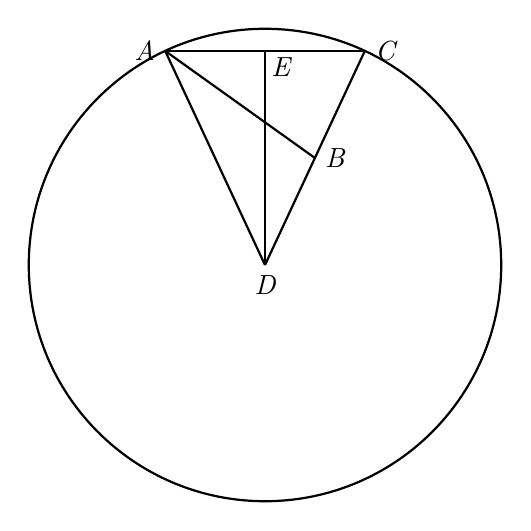
\begin{tikzpicture}[scale=1.5, thick, font=\itshape]
    % 1. 定义核心点坐标 (基于图像结构推算)
    \coordinate (D) at (0,0);               % 圆心 D
    \def\R{2}                               % 设置圆半径为 2
    \coordinate (A) at (115:\R);            % 点 A 在圆周上 (115度方向)
    \coordinate (C) at (65:\R);             % 点 C 在圆周上 (65度方向)
    
    % 2. 计算派生点
    % E 点为弦 AC 的中点 (垂足)
    \coordinate (E) at ($(A)!0.5!(C)$);     
    
    % B 点位于半径 DC 上，且满足 A, B 连线
    % 此处模拟图像位置，设定 B 在 DC 段约 0.4 比例处
    \coordinate (B) at ($(D)!0.5!(C)$);     

    % 3. 绘制图形边界
    % 绘制圆 (为了模仿原图，可以绘制带缺口的圆弧或全圆)
    \draw (D) circle (\R);
    
    % 绘制三角形和线段
    \draw (A) -- (C);                       % 弦 AC
    \draw (D) -- (A);                       % 半径 DA
    \draw (D) -- (C);                       % 半径 DC
    \draw (D) -- (E);                       % 线段 DE (垂直于 AC)
    \draw (A) -- (B);                       % 线段 AB

    
    \node[left] at (A) {A};
    \node[right] at (C) {C};
    \node[below] at (D) {D};
    \node[right] at (B) {B};
    \node[below right=-2pt] at (E) {E};



\end{tikzpicture}
\end{document}